% ================================ L'IMPLEMENTAZIONE ====================================

\chapter{L'implementazione}

%TODO: Implementazione in C++
%TODO: Con gui e command line o solo gui.

%TODO: Volendo anche Java?

%TODO: Presenterò/Mostrerò due implementazioni una fatta specificamente per questo progetto in C++ e un'altra in Java che avevo fatto per altri progetti.
%TODO: Quella in C++ sarà più completa rispetto di quella in Java.

% =======================================================================================

% ---------------------------- SECTION: INTRODUZIONE ------------------------------------

\section{Introduzione}

\textsf{\small In questo capitolo, presenterò due implementazioni, una elaborata esclusivamente per questo progetto in C++ e un'altra in Java che avevo creato per altri progetti universitari. Quella in C++ risulterà più completa rispetto a quella in Java.} %TODO: In questo capitolo, presenterò due implementazioni, una elaborata esclusivamente per questo progetto in C++ e un'altra in Java che avevo creato per altri progetti universitari. Quella in C++ risulterà più completa rispetto a quella in Java.

% ---------------------------- SECTION: IMPLEMENTAZIONE IN C++ --------------------------

\section{Implementazione in C++}

\textsf{\small Ho adottato C++23 per questo progetto. In esso sono presenti una interfaccia grafica e una applicazione da linea di comando, entrambe hanno le stesse operazioni.} %TODO: Ho adottato C++23 per questo progetto. In esso sono presenti una interfaccia grafica e una applicazione da linea di comando, entrambe hanno le stesse operazioni.

\textsf{\small Inanzittutto, esibirò, le funzioni riguardanti la matematica di Galois di cui mi sono avvalso.}

%TODO: Inanzittutto, esibirò, le funzioni riguardanti la matematica di Galois di cui mi sono avvalso.

\subsection{Matematica di Galois}

%TODO: Aggiungere immagine IRREDUCIBLE POLYNOMIAL?

\textsf{\small Riguardo alla matematica nel campo di Galois, ho adoperato tre funzioni: una che implementa l'addizione e la sottrazione, una per la moltiplicazione e una per generare le costanti di round.} %TODO: 

\textsf{\small Nel campo di Galois, sia l'addizione che la sottrazione sono semplicemente un'operazione di XOR. Questa funzione prende due parametri x ed y di tipo \emph{uint8\_t} (che corrisponde a un \emph{unsigned char}) e restituisce lo XOR tra essi.}

\begin{figure}[H]
	\centering
	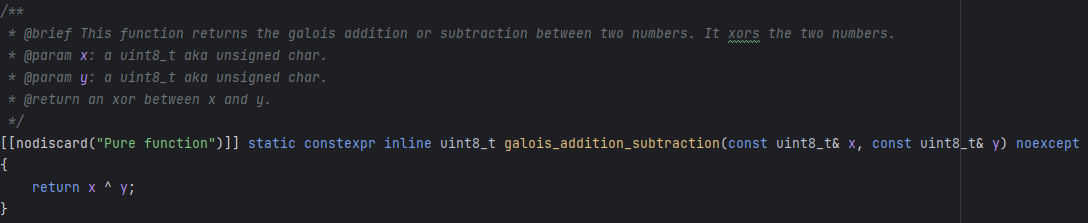
\includegraphics[width=1\textwidth, height=1\textheight, keepaspectratio]{./images/code/cpp/galois_math/galois_addition_subtraction.PNG}
	\caption{Addizione e sottrazione nel campo di Galois}
	\label{fig:galois_addition_subtraction}
\end{figure}

\textsf{\small \emph{galois\_multiplication()} prende due \emph{uint8\_t} come parametri e restituisce la moltiplicazione tra questi nel campo di Galois.}

\textsf{\emph{static constexpr} indicano che la funzione può essere eseguita a compile time. \emph{noexcept} indica che la funziona non lancia eccezioni. \emph{[[nodiscard]]} indica che il risultato che viene restituito non può essere ignorato, ma deve essere utilizzato.}

%TODO: Aggiungere reference alla parte nel capitolo della Matematica o aggiungere breve spiegazione.

\textsf{\small Facciamo un loop su ogni bit del byte e verifichiamo se il secondo valore \emph{y} ha il bit meno significativo attivo (y \& 0x01) allora aggiungiamo \emph{x} (ovvero eseguiamo uno XOR) al risultato. Dopodiché verifichiamo se il bit più significativo \emph{high\_bit} è attivo in \emph{x}. Poi ruotiamo x di 1. Se l'\emph{high\_bit} è \emph{true} eseguiamo uno XOR tra x e il polinomio irriducibile \emph{IRREDUCIBLE\_POLYNOMIAL}, ovvero $0x1\text{B}$. Infine ruotiamo il secondo valore di 1 per ruotarlo a destra. Poi restituiamo il risultato finale delle operazioni.}

\begin{figure}[H]
	\centering
	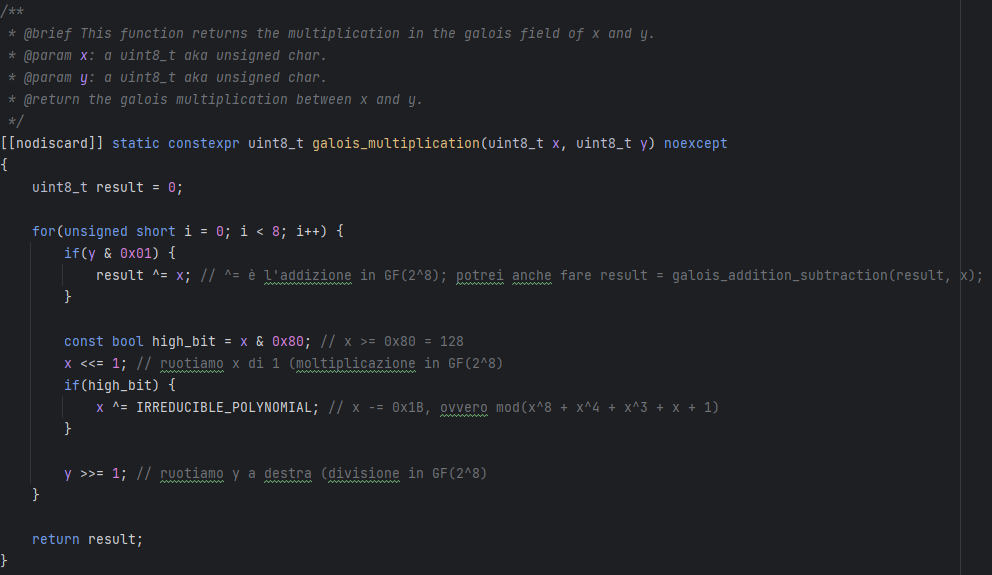
\includegraphics[width=1\textwidth, height=1\textheight, keepaspectratio]{./images/code/cpp/galois_math/galois_multiplication.PNG}
	\caption{Moltiplicazione nel campo di Galois}
	\label{fig:galois_multiplication}
\end{figure}

\textsf{\small \emph{round\_constant\_generator(const uint8\_t\& x)} prende un numero in input e restituisce la round constant.} %TODO:

\textsf{\small Questa funzione è utilizzata per generare la round constant.}
\textsf{\small L'algoritmo di questa funzione è il seguente: }

\begin{itemize}
	\item \textsf{\small il round\_constant(1) = 1.}
	\item \textsf{\small round\_constant(i) = $2 \cdot \text{round\_constant}(i - 1) \text{se round\_constant(i - 1) < 0x80}$}
	\item \textsf{\small round\_constant($2 \cdot \text{round\_constant(i - 1)}$) $ \oplus \hspace{0.3mm} \text{0x11B } \ge 0x80$ }
\end{itemize}

\begin{figure}[H] %TODO: update.
	\centering
	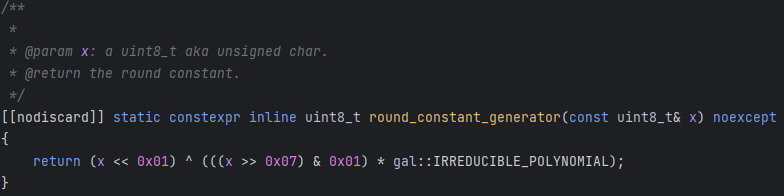
\includegraphics[width=1\textwidth, height=1\textheight, keepaspectratio]{./images/code/cpp/galois_math/round_constant_generator.PNG}
	\caption{Generatrice delle costanti di round}
	\label{fig:round_constant_generator}
\end{figure}

%TODO: Come prima cosa mostrerò l'implementazione dell'algoritmo di AES con tutte le varie operazioni all'interno di ogni round di AES, ovvero: add round key, sub bytes, shift rows e mix columns. Dopodiché presenterò la parte di Key Expansion, ovvero come vengono ottenute le chiavi per ogni round, anch'esso composto da queste fasi: rot word, sub word, rcon.

%\subsection{Cifratura} %TODO: uncomment?

\subsection{Add Round Key}

\textsf{\small Nella fase di \emph{add\_round\_key()} la chiave di round viene aggiunta alla matrice di stato.}

\textsf{\small La funzione prende la matrice di stato 4x4 (formata da due std::array di grandezza BLOCK\_WORDS che indica il numero di words in un blocco, ovvero 4) e la chiave del round come puntatore e le aggiunge.}

\begin{figure}[H]
	\centering
	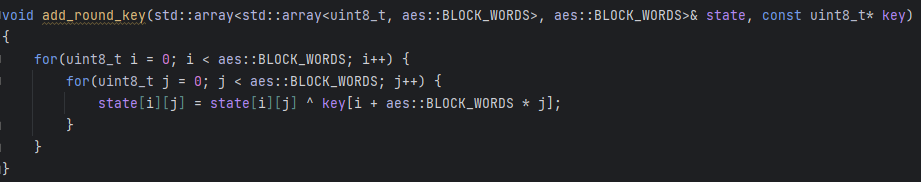
\includegraphics[width=1\textwidth, height=1\textheight, keepaspectratio]{./images/code/cpp/encryption/add_round_key.PNG}
	\caption{Add Round Key}
	\label{fig:add_round_key}
\end{figure}

\subsection{Sub Bytes}

\textsf{\small Nella funzione \emph{sub\_bytes} ogni byte della matrice di stato viene sostituito con quelli presenti nella S-BOX.}

\textsf{\small Quindi, nella funzione viene passata la matrice di stato come reference, quindi tutti le modifiche verranno applicate anche all'esterno della funzione e poi viene eseguito un loop e ogni elemento viene sostituito con il corrispettivo della S-BOX.}

\begin{figure}[H]
	\centering
	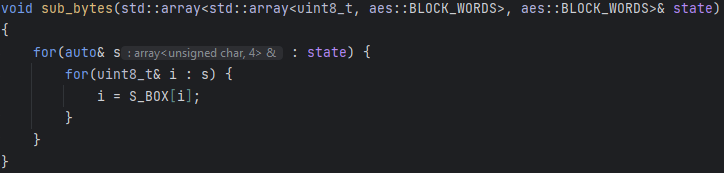
\includegraphics[width=1\textwidth, height=1\textheight, keepaspectratio]{./images/code/cpp/encryption/sub_bytes.PNG}
	\caption{Sub Bytes}
	\label{fig:sub_bytes}
\end{figure}

\subsection{Shift Rows}

\textsf{\small Nel passaggio di \emph{shift rows} le righe della matrice di stato verranno \emph{shiftate} di una posizione la seconda riga, di due posizione la terza e di tre la quarta.}

\textsf{\small Per fare questo ci avvaliamo di due funzioni, una \emph{shift\_row} per shiftare effettivamente le righe e nell'altra \emph{shift\_rows} per chiamare la precedente funzione per shiftare delle posizioni stabilite.}

%TODO: aggiungere altro?

\begin{figure}[H]
	\centering
	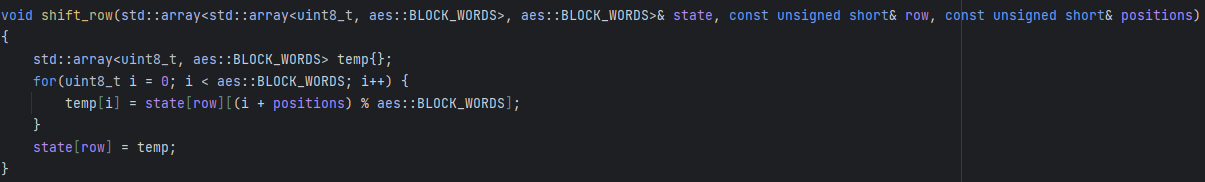
\includegraphics[width=1\textwidth, height=1\textheight, keepaspectratio]{./images/code/cpp/encryption/shift_row.PNG}
	\caption{Shift Row}
	\label{fig:shift_row}
\end{figure}

\textsf{\small } %TODO:

\begin{figure}[H]
	\centering
	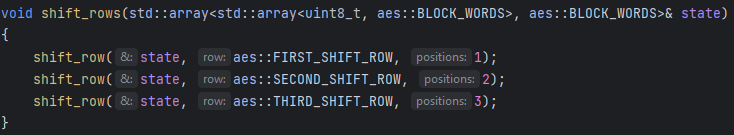
\includegraphics[width=1\textwidth, height=1\textheight, keepaspectratio]{./images/code/cpp/encryption/shift_rows.PNG}
	\caption{Shift Rows}
	\label{fig:shift_rows}
\end{figure}

\subsection{Mix Columns}

\textsf{\small La procedura \emph{mix\_columns} prende in input la matrice di stato, mescola i suoi bytes.} %TODO:

%TODO: Aggiungere altro.

\begin{figure}[H]
	\centering
	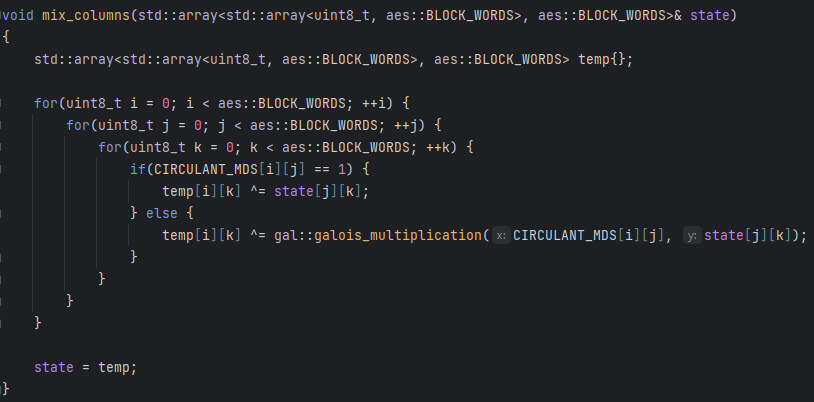
\includegraphics[width=1\textwidth, height=1\textheight, keepaspectratio]{./images/code/cpp/encryption/mix_columns.PNG}
	\caption{Mix Columns}
	\label{fig:mix_columns}
\end{figure}

%TODO: funzioni di decifrazione?

\subsection{Key Expansion}

\textsf{\small In questa funzione vengono generate le altre chiavi dei rounds a partire dalla prima chiave. Gli viene passata un array con la chiave, una word e la tipologia di AES: 128, 192 o 256.} %TODO:

\textsf{\small Dopodiché eseguiamo le operazioni di: \emph{rot\_word}, \emph{sub\_word}, e \emph{rcon}. Dopodiché viene eseguito uno XOR tra la chiave e il rcon. Dopodiché si continua a eseguire uno XOR con le chiavi precedenti.}

%TODO: Aggiungere altro.

\begin{figure}[H]
	\centering
	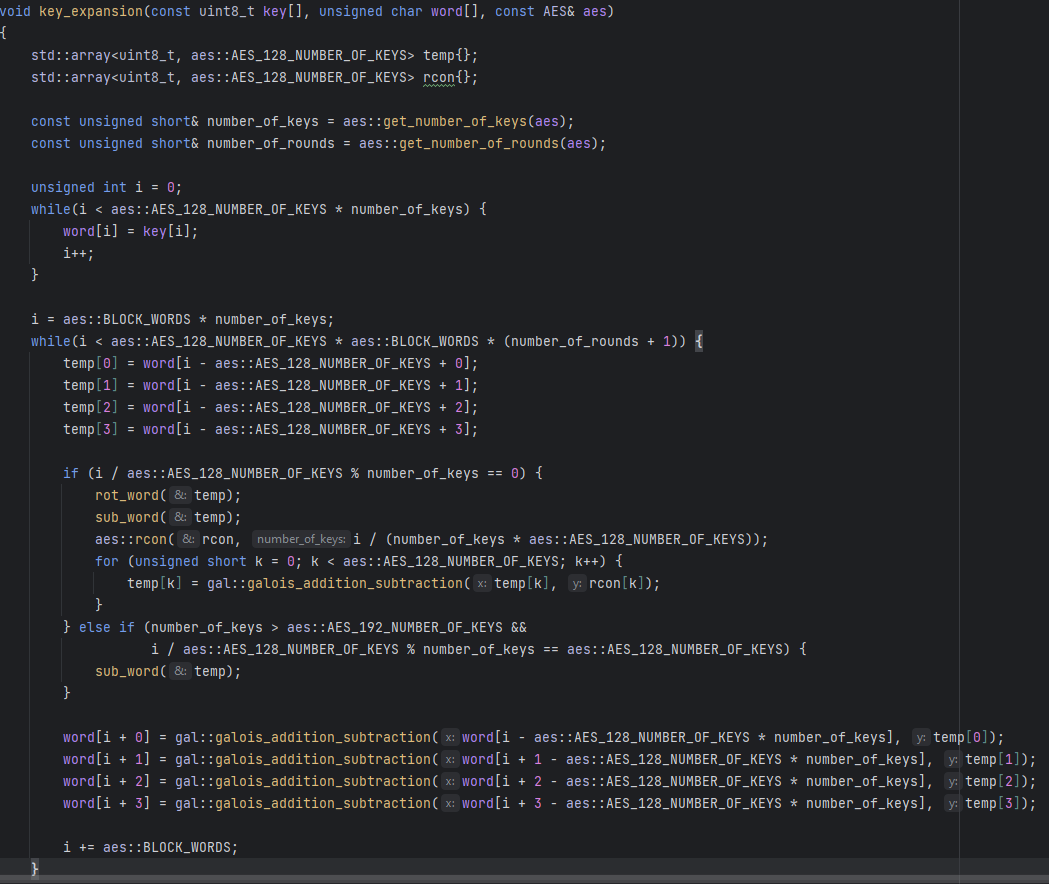
\includegraphics[width=1\textwidth, height=1\textheight, keepaspectratio]{./images/code/cpp/key_expansion/key_expansion.PNG}
	\caption{Key Expansion}
	\label{fig:key_expansion_code}
\end{figure}

\subsubsection{Rot Word}

\begin{figure}[H]
	\centering
	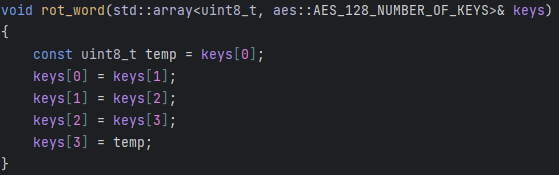
\includegraphics[width=1\textwidth, height=1\textheight, keepaspectratio]{./images/code/cpp/key_expansion/rot_word.PNG}
	\caption{Rot Word}
	\label{fig:rot_word}
\end{figure}

\textsf{\small In questa operazione ogni byte (word di 32 bits, ovvero 4 bytes) viene ruotato di 1 posizione.} %TODO: Aggiungere altro.

\subsubsection{Sub Word}

\begin{figure}[H]
	\centering
	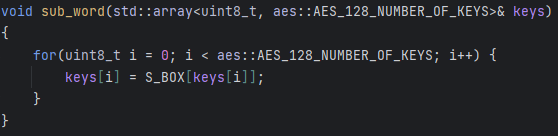
\includegraphics[width=1\textwidth, height=1\textheight, keepaspectratio]{./images/code/cpp/key_expansion/sub_word.PNG}
	\caption{Sub Word}
	\label{fig:sub_word}
\end{figure}

\textsf{\small Nella procedura \emph{sub\_word()} ogni byte della chiave viene sostituita con quella della S-BOX.} %TODO:

\subsubsection{Rcon}

\begin{figure}[H]
	\centering
	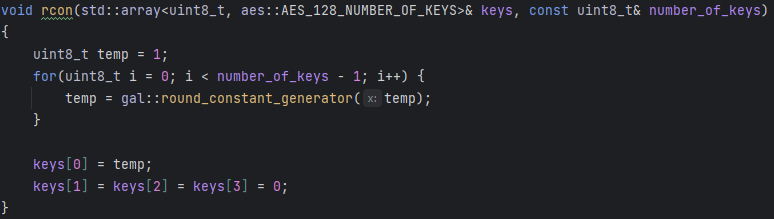
\includegraphics[width=1\textwidth, height=1\textheight, keepaspectratio]{./images/code/cpp/key_expansion/rcon.PNG}
	\caption{Rcon}
	\label{fig:rcon}
\end{figure}

\textsf{\small Nella funzione \emph{rcon}, le \emph{round constants} vengono generate attraverso una funzione ricorsiva.} %TODO:

\subsubsection{Xor Blocks} %TODO: uncomment?

\textsf{\small Con questa funzione eseguiamo uno XOR per ogni bit \emph{i} tra i blocchi x e y e assegniamo il risultato a ogni bit del blocco z. }

\textsf{\small Il loop viene eseguito in base alla grandezza del blocco.}

\begin{figure}[H]
	\centering
	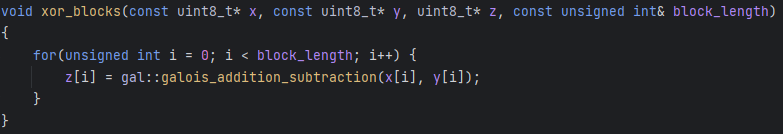
\includegraphics[width=1\textwidth, height=1\textheight, keepaspectratio]{./images/code/cpp/key_expansion/xor_blocks.PNG}
	\caption{Xor Blocks}
	\label{fig:xor_blocks}
\end{figure}

%\textsf{\small } %TODO:

\subsection{Modes}

\textsf{\small } %TODO:

%TODO: subsection: Modes con codice? Questo si potrebbe fare.

\subsubsection{ECB}

\textsf{\small ECB è la modalità più semplice e anche quella che non dovrebbe mai essere usata.} %TODO: aggiungere reference alla spiegazione della modalità.

\textsf{\small In questa modalità, semplicemente, ogni blocco viene cifrato com'è. Nessun vettore di inizializzazione viene utilizzato. Lo stesso input genererà lo stesso identico output.}

\textsf{\small Questa modalità inoltre accetta solo blocchi divisibili per 16, questo viene garantito attraverso la funzione \emph{verify\_length()} che verifica e lancia un'eccezione altrimenti.}

\begin{figure}[H]
	\centering
	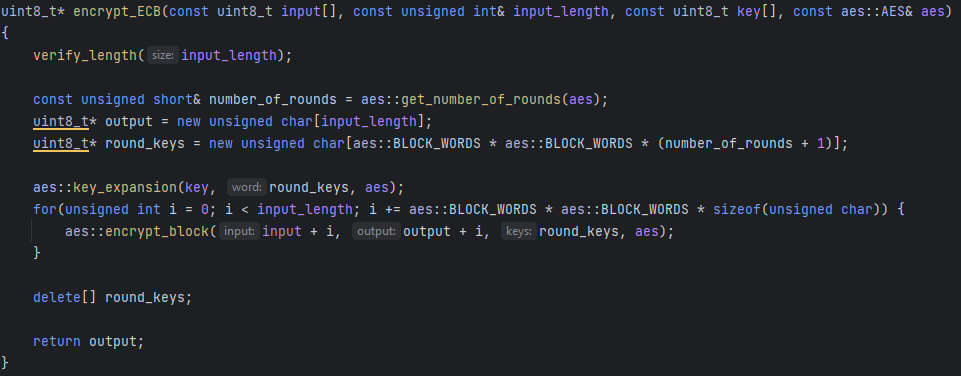
\includegraphics[width=1\textwidth, height=1\textheight, keepaspectratio]{./images/code/cpp/modes/encrypt_ECB.PNG}
	\caption{Cifratura ECB}
	\label{fig:encrypt_ECB}
\end{figure}

\textsf{\small Per la decifrazione è lo stesso procedimento, ma inverso. } %TODO:

\begin{figure}[H]
	\centering
	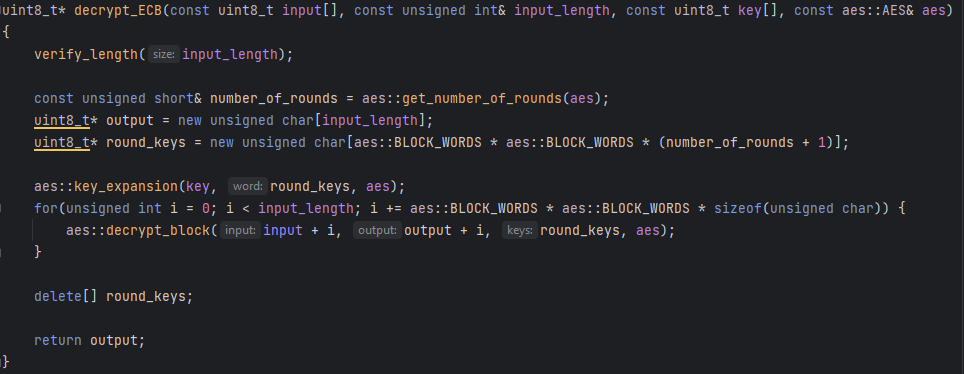
\includegraphics[width=1\textwidth, height=1\textheight, keepaspectratio]{./images/code/cpp/modes/decrypt_ECB.PNG}
	\caption{Decifrazione ECB}
	\label{fig:decrypt_ECB}
\end{figure}

\subsubsection{CBC}

\textsf{\small CBC è la modalità di chaining, in cui viene utilizzato un IV (initialization vector) per aggiungere casualità e viene eseguito uno XOR tra il messaggio in chiaro e il testo cifrato.} %TODO:

\begin{figure}[H]
	\centering
	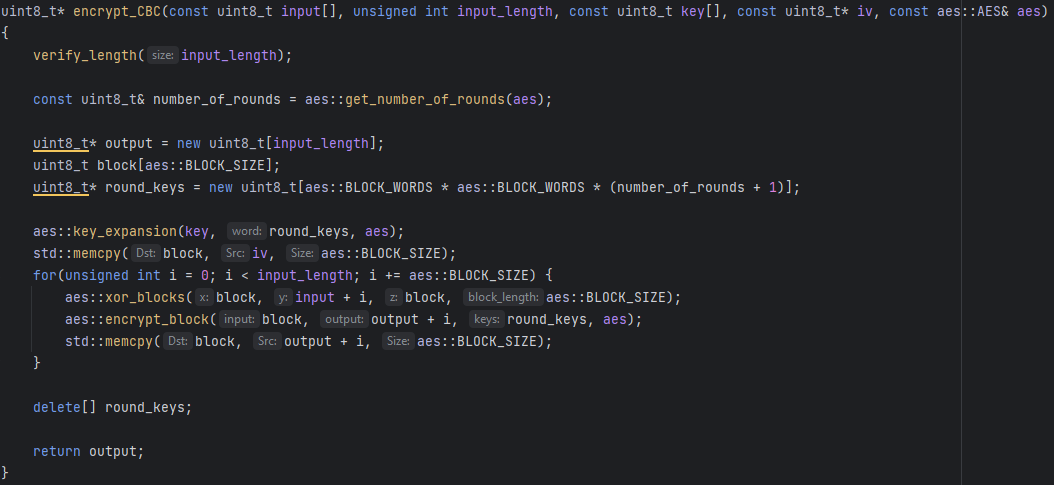
\includegraphics[width=1\textwidth, height=1\textheight, keepaspectratio]{./images/code/cpp/modes/encrypt_CBC.PNG}
	\caption{Cifratura CBC}
	\label{fig:encrypt_CBC}
\end{figure}

\textsf{\small } %TODO:

\begin{figure}[H]
	\centering
	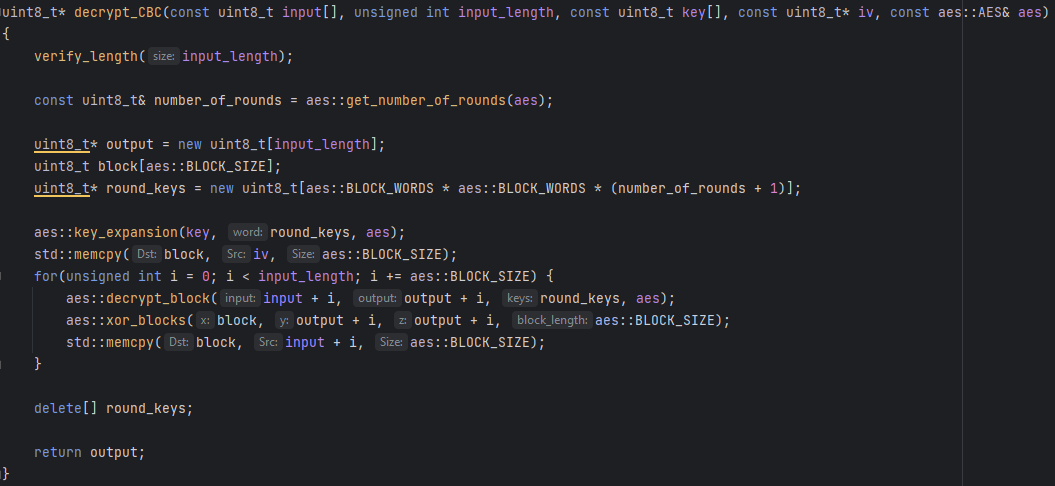
\includegraphics[width=1\textwidth, height=1\textheight, keepaspectratio]{./images/code/cpp/modes/decrypt_CBC.PNG}
	\caption{Decifrazione CBC}
	\label{fig:decrypt_CBC}
\end{figure}

\subsubsection{CFB}

\textsf{\small In queste funzioni, innanzitutto, verifico che la lunghezza dell'input sia divisibile per 16, poi ottengo il numero di rounds in base a quale AES stiamo utilizzando. Imposto l'output, il blocco, il blocco cifrato e le chiavi di rounds che ottengo dalla key\_expansion. Dopodiché cifro il blocco, eseguo uno XOR tra il plaintext e il blocco cifrato. Infine restituisco l'output.} %TODO:

\begin{figure}[H]
	\centering
	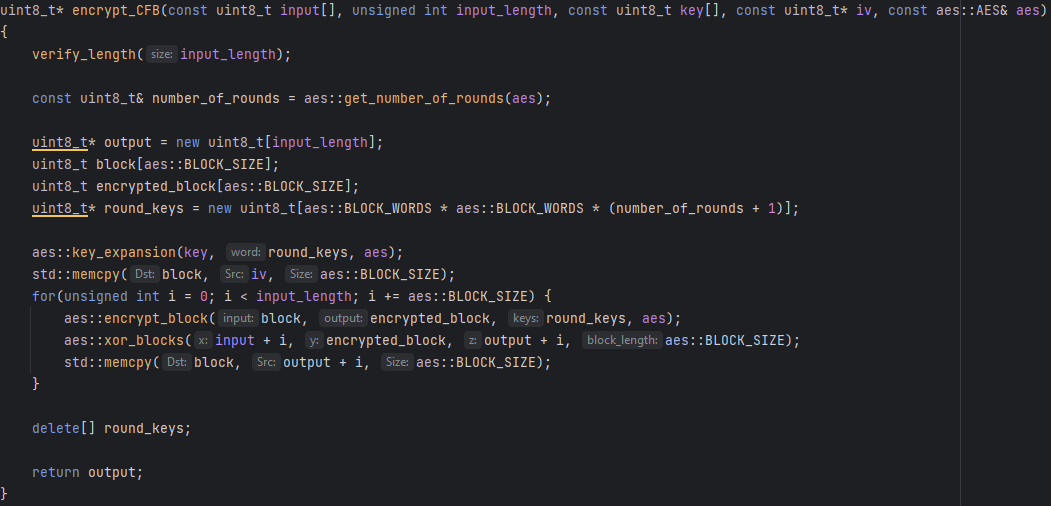
\includegraphics[width=1\textwidth, height=1\textheight, keepaspectratio]{./images/code/cpp/modes/encrypt_CFB.PNG}
	\caption{Cifratura CFB}
	\label{fig:encrypt_CFB}
\end{figure}

\textsf{\small }

\begin{figure}[H]
	\centering
	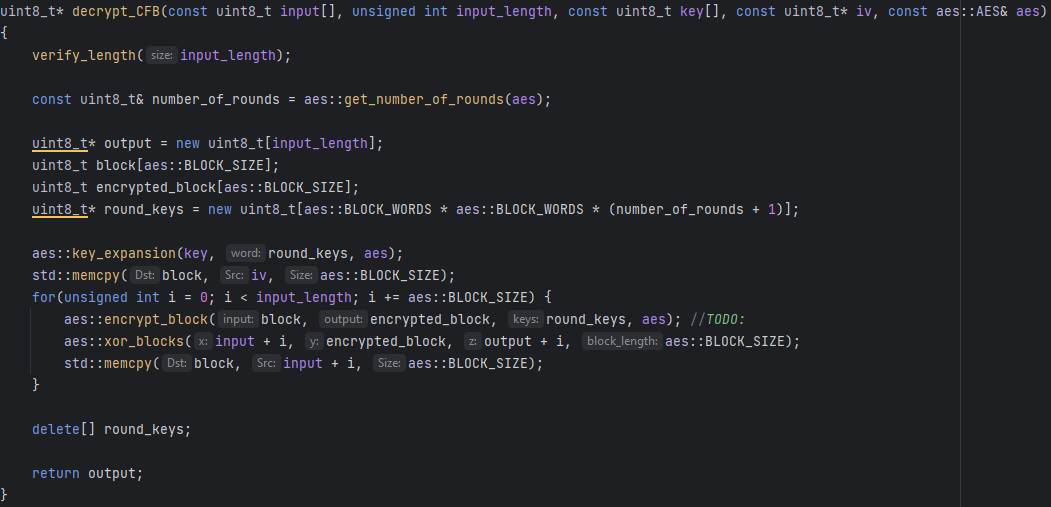
\includegraphics[width=1\textwidth, height=1\textheight, keepaspectratio]{./images/code/cpp/modes/decrypt_CFB.PNG}
	\caption{Decifrazione CFB}
	\label{fig:decrypt_CFB}
\end{figure}

\subsection{Paddings}

\textsf{\small Il padding viene utilizzato per aggiungere dei caratteri prestabiliti alla fine di un messaggio. Abbiamo due funzioni, una per aggiungere il padding, add\_padding e una per rimuoverlo, remove\_padding. Entrambe queste funzioni richiedono il messaggio da cui vogliamo aggiungere/rimuovere il padding e quale tipologia di padding applicare.} %TODO:

\textsf{\small Otteniamo, innanzitutto, il resto per vedere se il messaggio è perfettamente divisibile del BLOCK\_SIZE, ovvero 16 oppure no. Dopodiché calcoliamo la lunghezza mancante, sottraendo il BLOCK\_SIZE al resto.}

\begin{figure}[H]
	\centering
	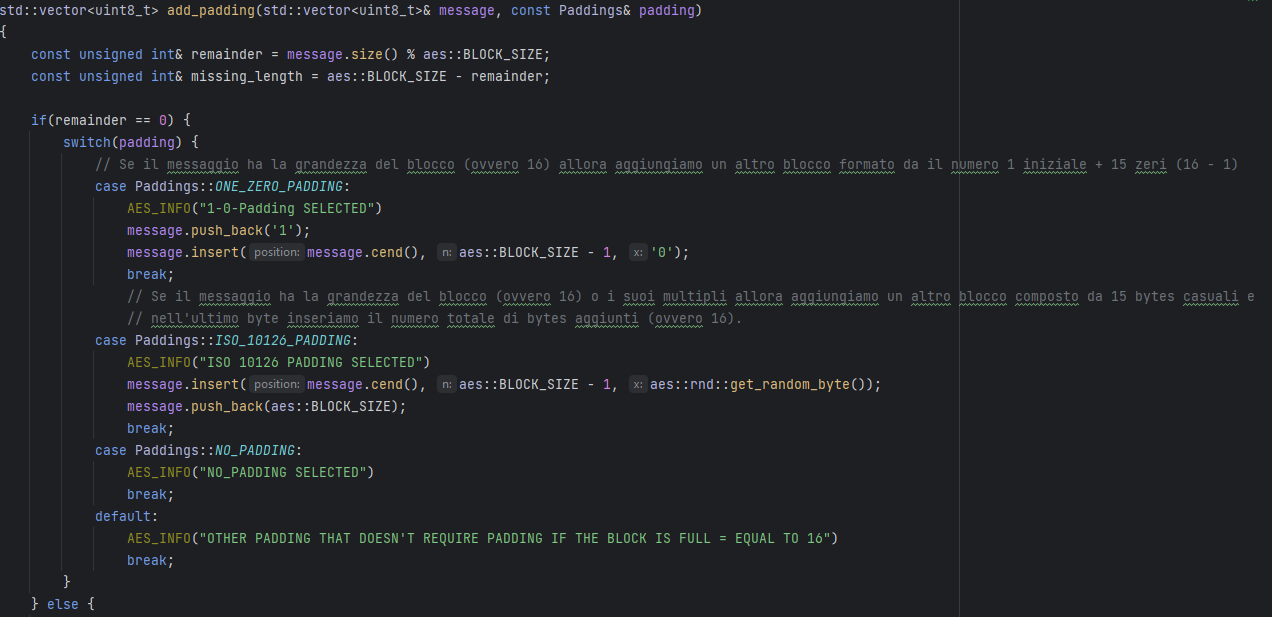
\includegraphics[width=1\textwidth, height=1\textheight, keepaspectratio]{./images/code/cpp/padding/add_padding0.PNG}
	\caption{Aggiunta del padding (1/2)}
	\label{fig:add_padding0}
\end{figure}

\textsf{\small Se il resto è 0, ovvero il blocco è formato da esattamente 16 caratteri, allora eseguiamo questo:}

\begin{itemize}
	\item \textsf{\small \textbf{1-0-Padding}: Aggiungiamo un ulteriore blocco di lunghezza 16, ove il primo elemento è il carattere '1' e il rimanente è composto da zeri.}
	\item \textsf{\small \textbf{ISO\_10126\_PADDING}: Aggiungiamo 15 caratteri casuali e nell'ultimo carattere inseriamo il numero di caratteri casuali aggiunti.}
	\item \textsf{\small \textbf{NO\_PADDING} o qualsiasi altro padding: non facciamo nulla.}
\end{itemize}

\begin{figure}[H]
	\centering
	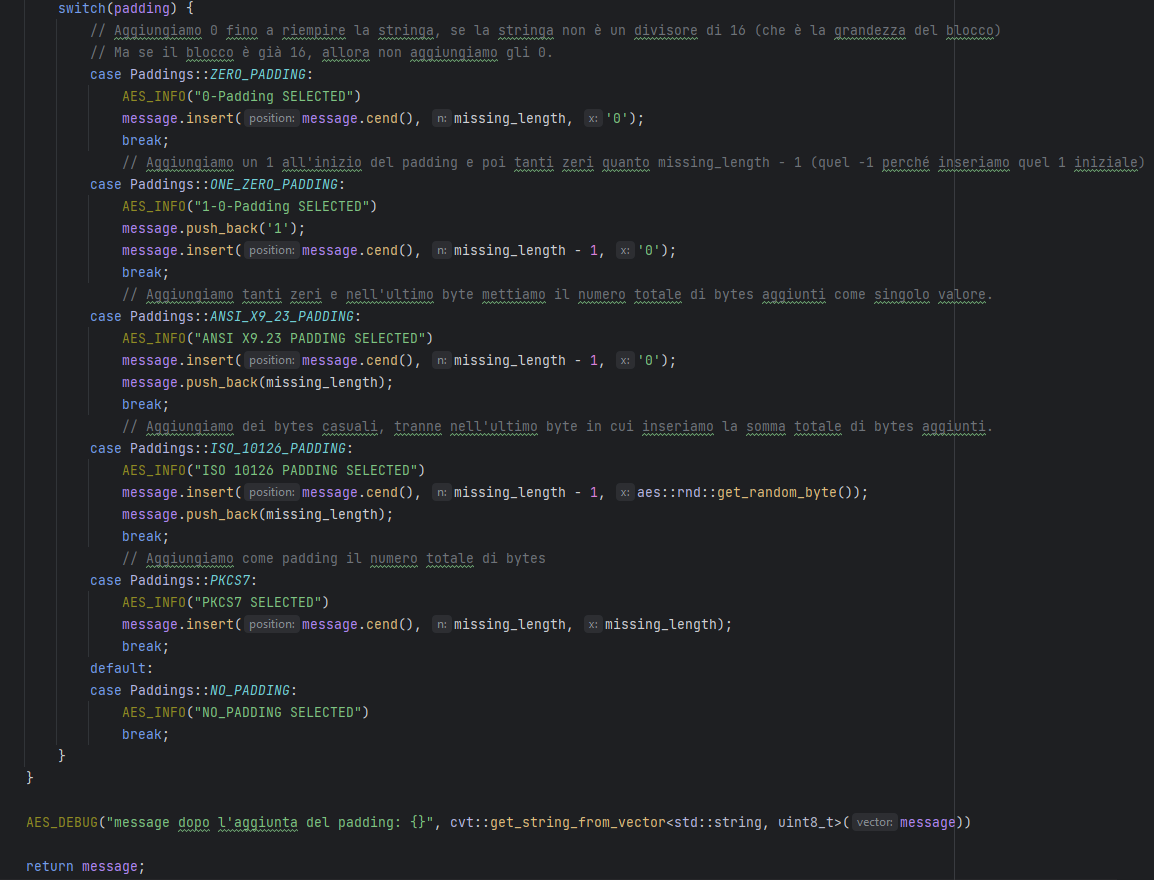
\includegraphics[width=1\textwidth, height=1\textheight, keepaspectratio]{./images/code/cpp/padding/add_padding1.PNG}
	\caption{Aggiunta del padding (2/2)}
	\label{fig:add_padding1}
\end{figure}

\textsf{\small Se il resto non è pari a 0, quindi il blocco non è pieno, non corrisponde a 16, allora eseguiamo:}

\begin{itemize}
	\item \textsf{\small \textbf{0-Padding}: Aggiungiamo tanti zeri quanti necessari per riempire il blocco.}
	\item \textsf{\small \textbf{1-0-Padding}: Aggiungiamo un 1 e poi tanti zeri quanti necessari per riempire il blocco.}
	\item \textsf{\small \textbf{ANSI\_X9\_23\_PADDING}: Aggiungiamo tanti zeri quanti necessari per riempire il blocco - 1, perché nell'ultimo byte inseriamo il numero degli zeri che abbiamo aggiunto.}
	\item \textsf{\small \textbf{ISO\_10126\_PADDING}: Aggiungiamo dei numeri casuali fino a riempire il blocco - 1, tranne che nell'ultimo byte in cui inseriamo il numero di bytes casuali aggiunti.}
	\item \textsf{\small \textbf{PKCS7}: Aggiungiamo il numero di bytes che mancano al riempire il blocco in tutti i blocchi rimanenti.}
	\item \textsf{\small \textbf{NO\_PADDING}: Non eseguiamo alcuna operazione al testo in chiaro.}
\end{itemize}

\begin{figure}[H]
	\centering
	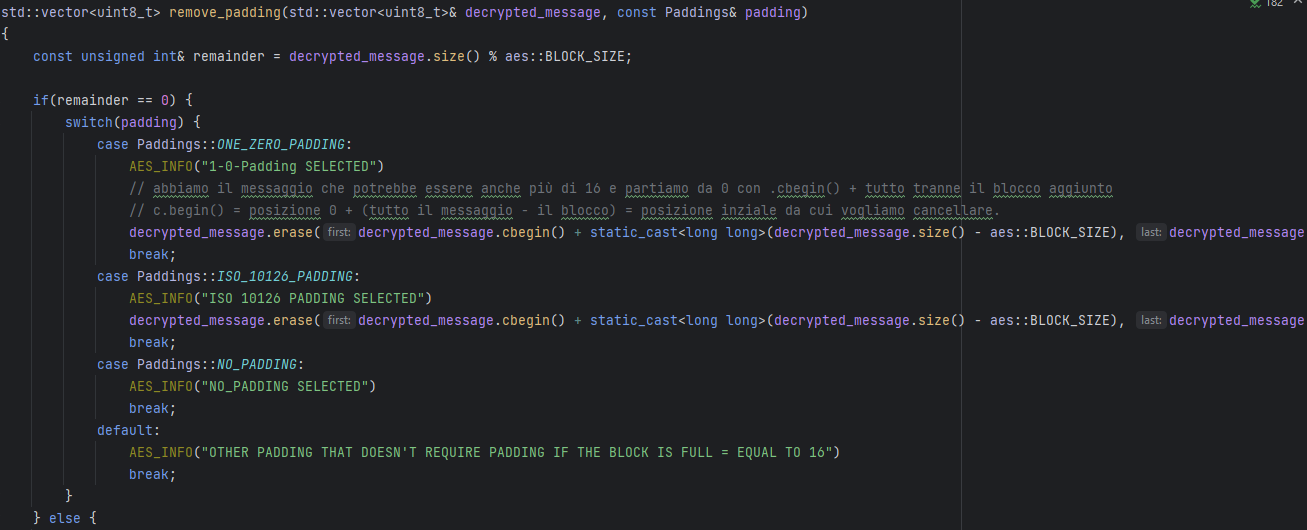
\includegraphics[width=1\textwidth, height=1\textheight, keepaspectratio]{./images/code/cpp/padding/remove_padding0.PNG}
	\caption{Rimozione del padding (1/2)}
	\label{fig:remove_padding0}
\end{figure}

\begin{figure}[H]
	\centering
	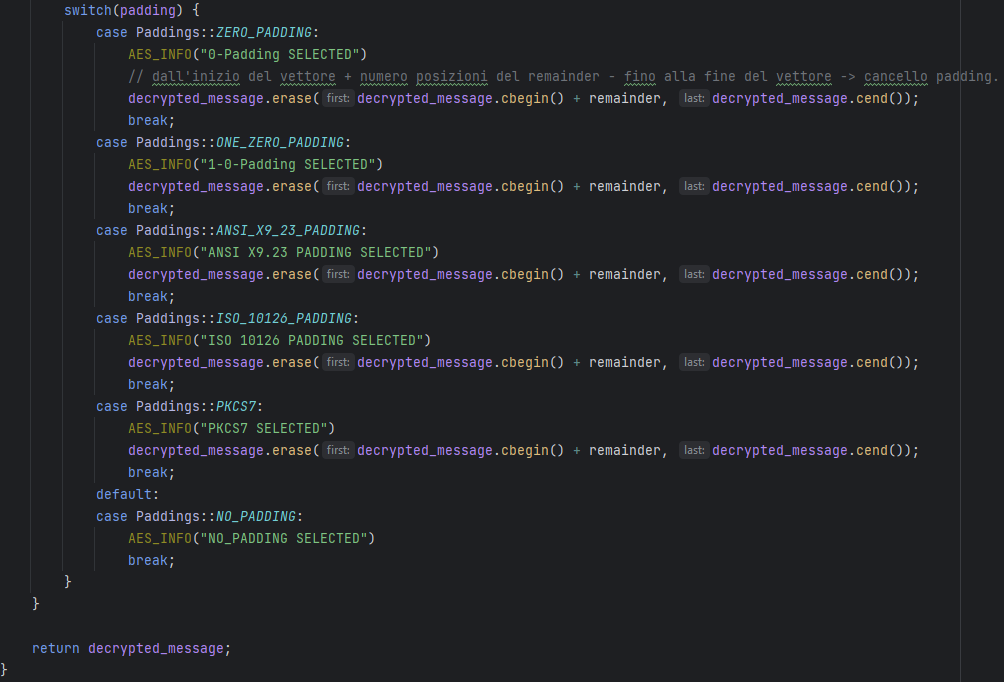
\includegraphics[width=1\textwidth, height=1\textheight, keepaspectratio]{./images/code/cpp/padding/remove_padding1.PNG}
	\caption{Rimozione del padding (2/2)}
	\label{fig:remove_padding1}
\end{figure}

\textsf{\small Per quanto riguarda la rimozione del padding, dal testo decifrato, è la stessa identica operazione dell'aggiunta, ma all'inverso, rimuovendo i bytes che avevamo aggiunto.} %TODO:

\subsection{API}

\textsf{\small Per poter interfacciarsi con tutte queste funzioni, ne sono presenti due: \emph{encrypt()} e \emph{decrypt()} che richiedono entrambe il messaggio (cifrato o in chiaro), la chiave, l'eventuale IV, opzionale, perché potrebbe non essere presente se si utilizza la modalità ECB, la tipologia di padding, la modalità e infine quale tipologia di AES.}

\subsubsection{Cifratura}

\textsf{\small Nella cifratura, viene aggiunto il padding chiamando \emph{add\_padding()} al messaggio in chiaro. Dopodiché, in base alla modalità scelta, viene restituito il messaggio cifrato.}

\begin{figure}[H]
	\centering
	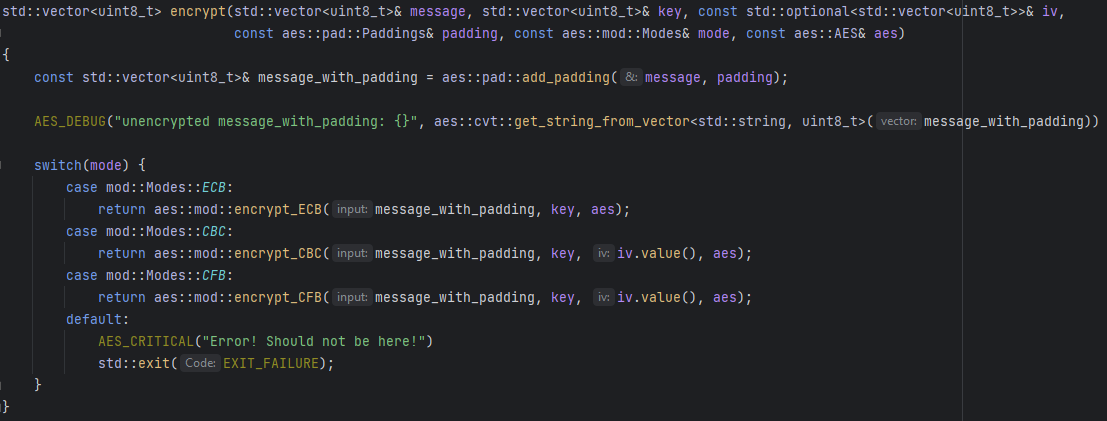
\includegraphics[width=1\textwidth, height=1\textheight, keepaspectratio]{./images/code/cpp/api/encrypt.PNG}
	\caption{Cifratura}
	\label{fig:encrypt}
\end{figure}

%TODO: encrypt_file?

\subsubsection{Decifratura}

\textsf{\small Nella decifratura, viene decifrato il messaggio in base alla modalità selezionata e dopodiché viene restituito il messaggio dopo la rimozione del padding, se presente.}

\begin{figure}[H]
	\centering
	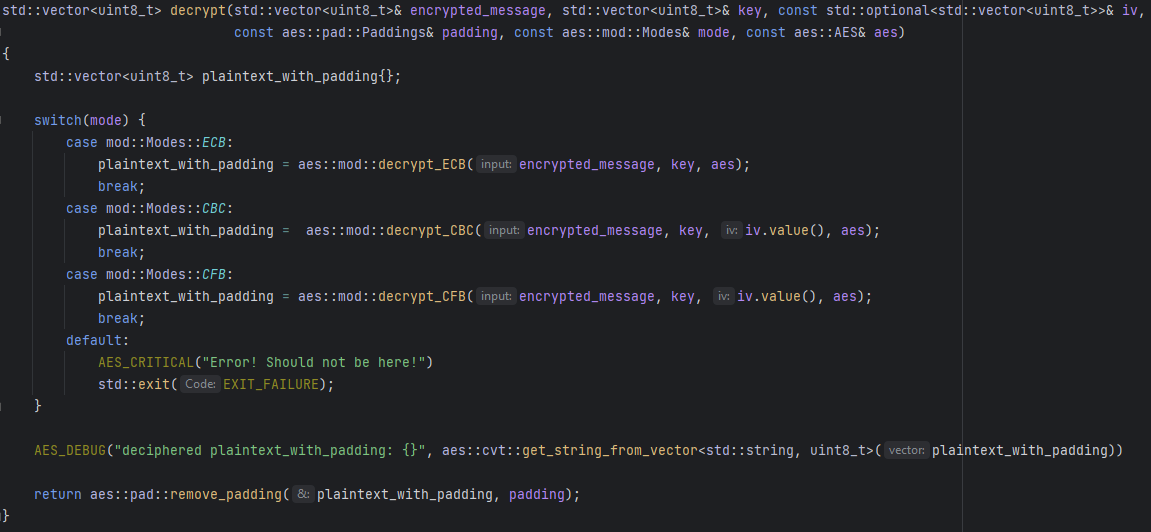
\includegraphics[width=1\textwidth, height=1\textheight, keepaspectratio]{./images/code/cpp/api/decrypt.PNG}
	\caption{Decifratura}
	\label{fig:decrypt}
\end{figure}

%TODO: decrypt_file?

%\textsf{\small } %TODO:

% ---------------------------- SECTION: IMPLEMENTAZIONE IN JAVA -------------------------

\section{Implementazione in Java}

\textsf{\small Per l'implementazione in Java, mi sono avvalso di Java 11 e ho usufruito delle librerie standard.} %TODO: 

\textsf{\small Ho definito, innanzitutto, delle variabili membro statiche, per definire la grandezza della chiave, quale algoritmo utilizzare, quale tipo di padding usufruire e altre inerenti l'iv e la salatura della password.}

\begin{figure}[H]
	\centering
	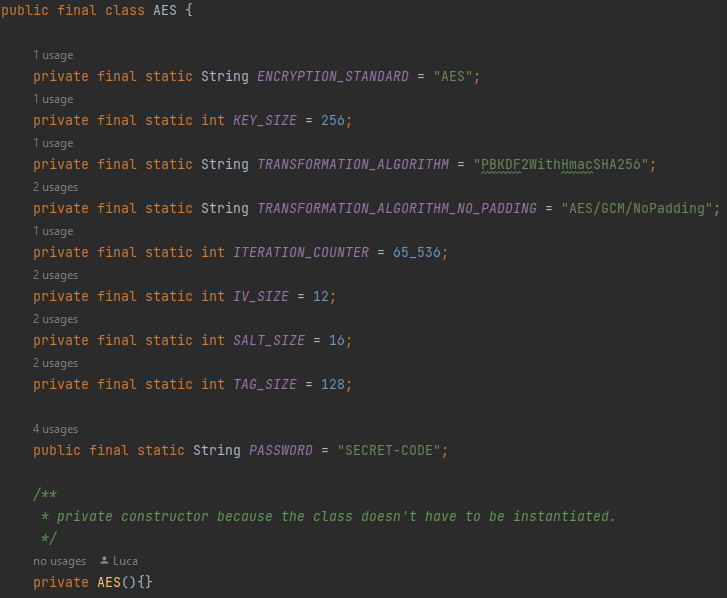
\includegraphics[width=1\textwidth, height=1\textheight, keepaspectratio]{./images/code/java/constructor_and_member_variables.PNG}
	\caption{Costruttore e variabili membre}
	\label{fig:constructor_and_member_variables}
\end{figure}

\textsf{\small Attraverso il metodo \emph{getRandomBytes()} otteniamo un Nonce.} %TODO: 

\begin{figure}[H]
	\centering
	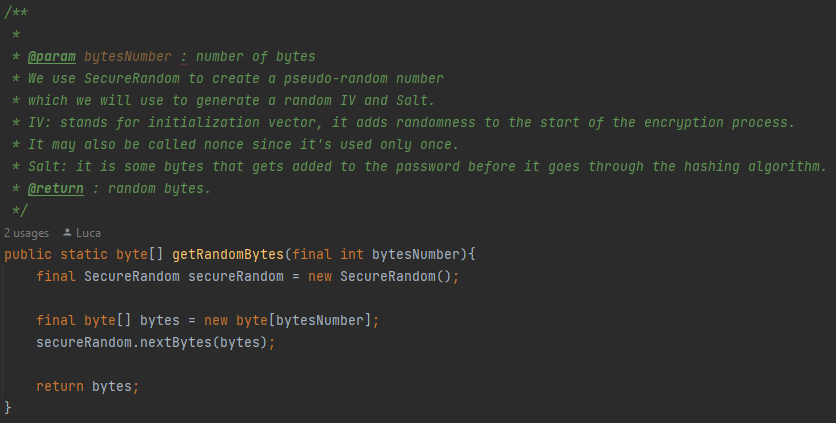
\includegraphics[width=1\textwidth, height=1\textheight, keepaspectratio]{./images/code/java/nonce_getRandomBytes.PNG}
	\caption{Nonce}
	\label{fig:nonce_getRandomBytes}
\end{figure}

\textsf{\small Col metodo \emph{getKeyFromPassword} otteniamo la chiave dalla password assieme alla salatura.} %TODO: 

\begin{figure}[H]
	\centering
	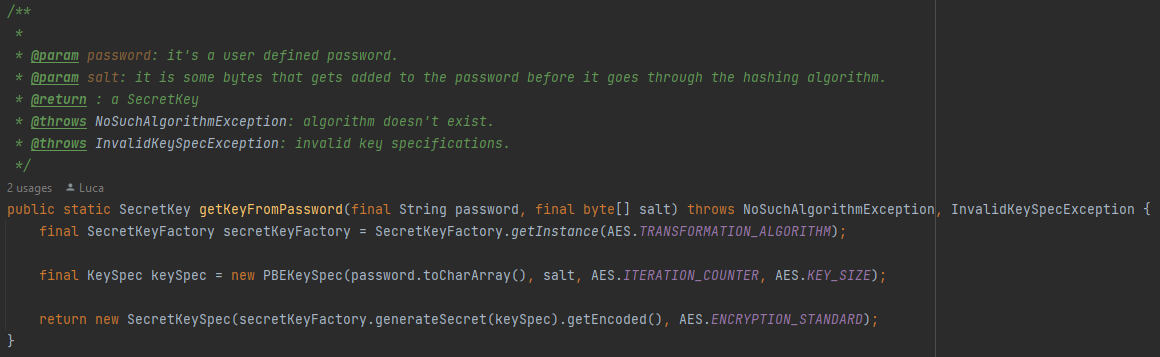
\includegraphics[width=1\textwidth, height=1\textheight, keepaspectratio]{./images/code/java/getKeyFromPassword.PNG}
	\caption{Password}
	\label{fig:getKeyFromPassword}
\end{figure}

\textsf{\small Nel metodo \emph{encrypt()} otteniamo la salatura e l'IV attraverso il metodo \emph{getRandomBytes()} e la chiave attraverso \emph{getKeyFromPassword()}. Dopodiché, inizializziamo il cifrario, cifriamo il messaggio e restituiamo il messaggio cifrato, assieme alla salatura e all'IV.} %TODO: 

\begin{figure}[H]
	\centering
	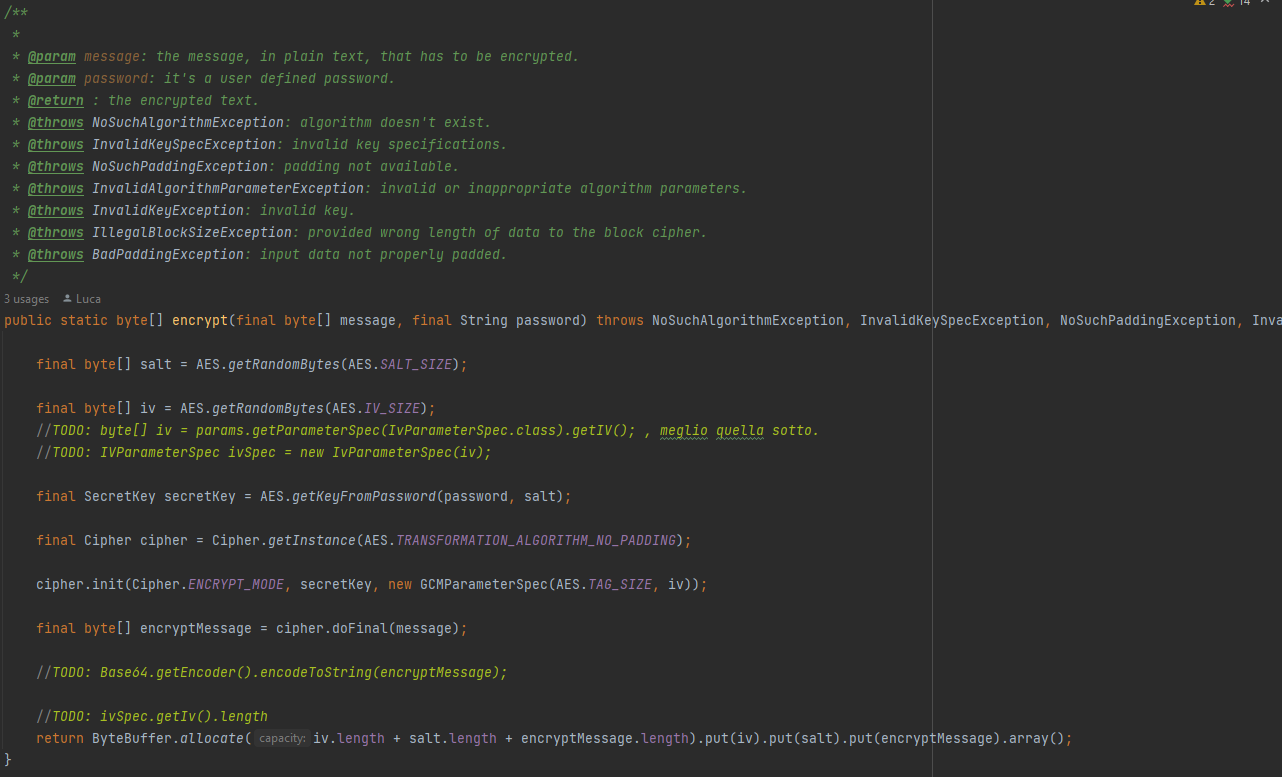
\includegraphics[width=1\textwidth, height=1\textheight, keepaspectratio]{./images/code/java/encrypt.PNG}
	\caption{Cifratura}
	\label{fig:encrypt_java}
\end{figure}

\textsf{\small Nel metodo \emph{decrypt()} otteniamo l'IV e il sale dal messaggio e recuperiamo la password, dopodiché inizializziamo il cifrario e decifriamo il messaggio.} %TODO: 

\begin{figure}[H]
	\centering
	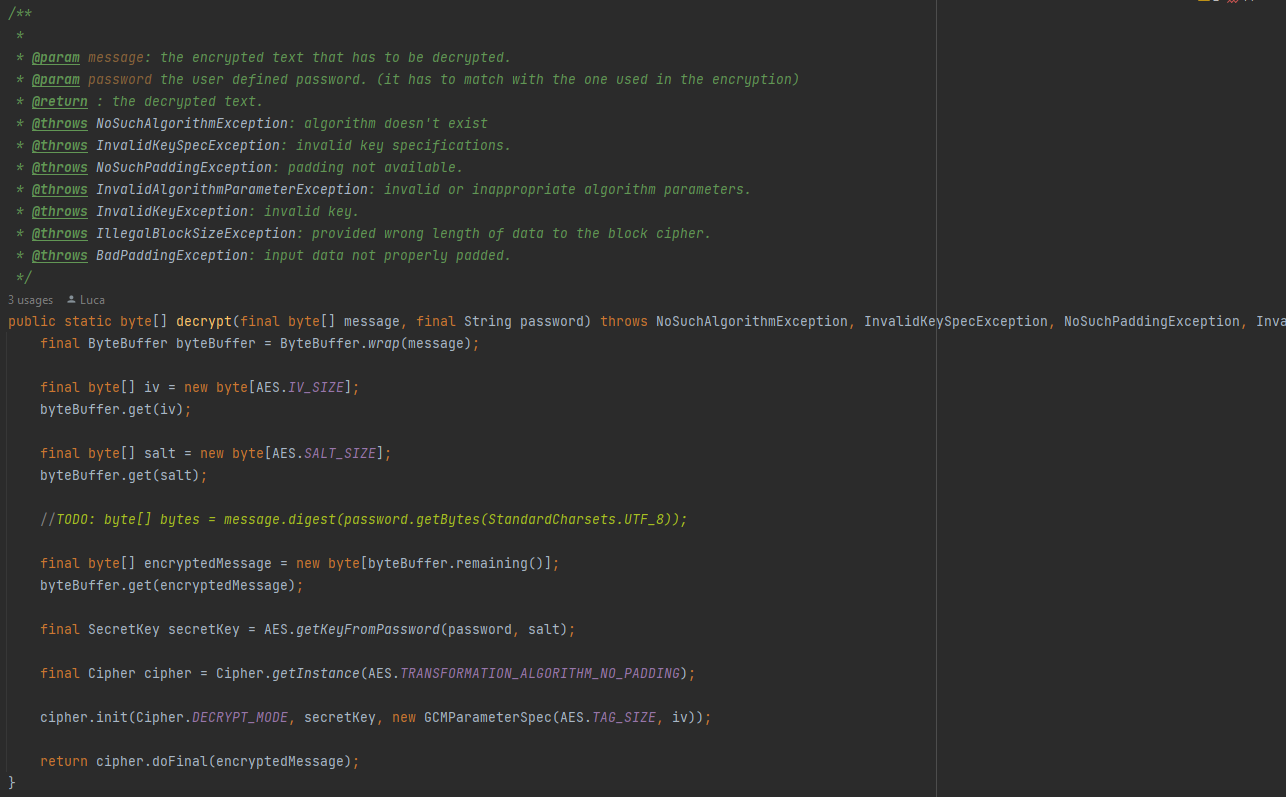
\includegraphics[width=1\textwidth, height=1\textheight, keepaspectratio]{./images/code/java/decrypt.PNG}
	\caption{Decifratura}
	\label{fig:decrypt_java}
\end{figure}

\textsf{\small In \emph{encryptFile} ci avvaliamo del metodo \emph{encrypt} per cifrare. Leggiamo i dati presenti nel file \emph{inputFilePath} e scriviamo il testo cifrato nel file \emph{outputFilePath}.} %TODO: 

\begin{figure}[H]
	\centering
	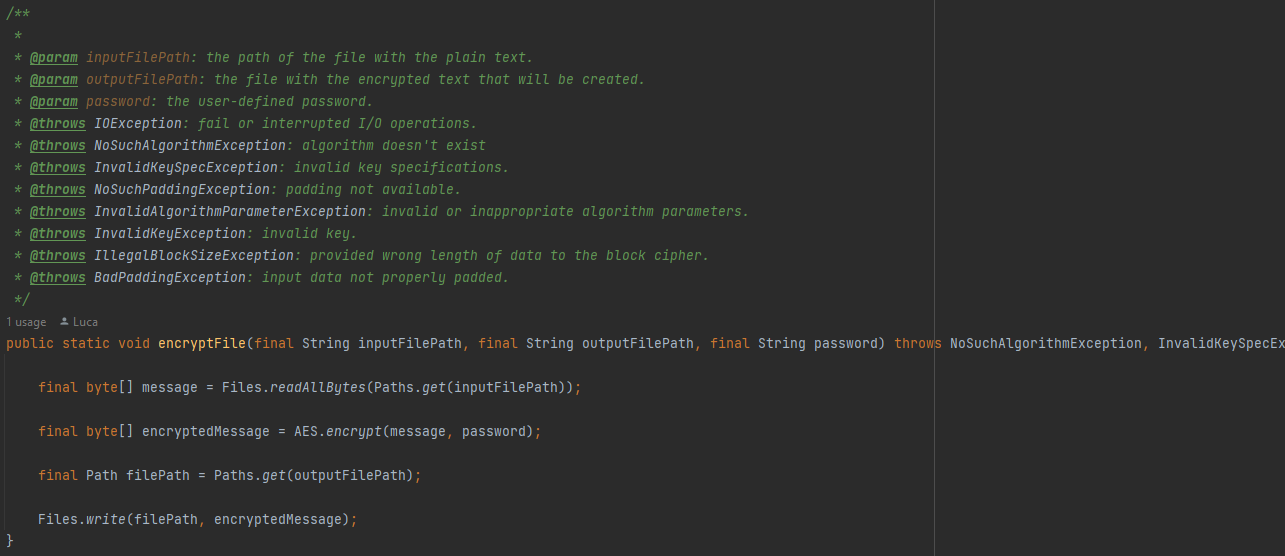
\includegraphics[width=1\textwidth, height=1\textheight, keepaspectratio]{./images/code/java/encryptFile.PNG}
	\caption{Funziona per la cifratura di un File}
	\label{fig:encryptFile}
\end{figure}

\textsf{\small Per \emph{decryptFile} adoperiamo il metodo \emph{decrypt} per decifrare il messaggio cifrato presente nella path indicata dalla variabile \emph{encryptedFilePath}.} %TODO: 

\begin{figure}[H]
	\centering
	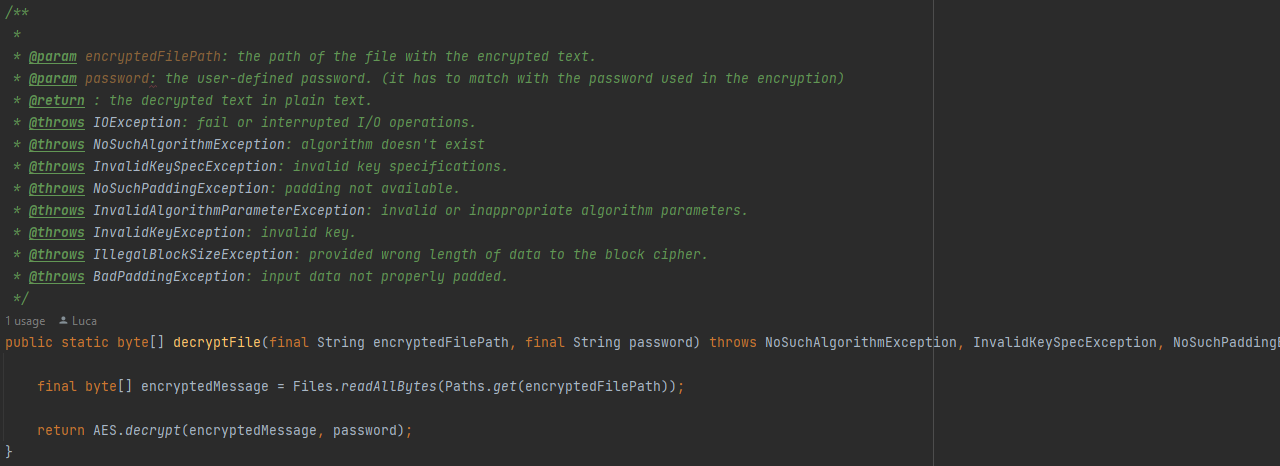
\includegraphics[width=1\textwidth, height=1\textheight, keepaspectratio]{./images/code/java/decryptFile.PNG}
	\caption{Funziona per la decifrazione di un File}
	\label{fig:decryptFile}
\end{figure}

%\textsf{\small } %TODO: 

% -------------------------------- FINE CAPITOLO ----------------------------------------